\documentclass[10pt, nofootinbib, twocolumn]{revtex4-1}
\usepackage{amsmath}
\usepackage{xparse}
\usepackage{graphicx}
\usepackage{hyperref}
\usepackage{color}
\usepackage{physics}
\usepackage{enumitem}
\usepackage{natbib}
\usepackage{booktabs}
\usepackage{float}
\usepackage{caption}
\usepackage{mathtools}
\usepackage{multirow}

\hypersetup{
    colorlinks=true,
    linkcolor=black,  
    citecolor=black,
    urlcolor=blue
}


\begin{document}
\vspace*{2\baselineskip}
\title{Project2 AST3310 - Energy Transportation Within Stars} 
\date{\today} \homepage{https://github.com/tirilsg/AST3310_Project2}       
\begin{abstract}
    \textit{A model for energy transportation, based on the previously developed model for energy production explained in the "Project 1: AST3310 report," is constructed in this report. It is programmed to be a python class taking parameters for luminosity, radius, temperature, density and mass of the surface of the star as arguments, and estimating how the essential, relevant parameters in intervals defined by variable step lengths from the surface towards the core. The sanity of the model is tested, and we get the largest relative error for the opacity $1.199\times 10^{-4}$. The sanity of the structure of the star is tested by creating cross section and temperature gradient plots. Another test is performed, using a specific set of surface defining variables and comparing expected and modelled parameter values. The structural implications of changing the initial parameters is tested and plotted, and an optimal set of variables defining the star is deliberated upon and retrieved ; $L_0=1.7$, $R_0=1$, $M_0=1.1$, $T_0=2\times5770$, $rho_0=70\times1.42\times 10^{-7}$. The simulation is ran using these surface-describing parameters, and a data analysis is presented in figures and compared to expected behaviours derived by theory. Both data analysis and sanity checks are grounds for the conclusion of a sufficiently accurate model.}
\end{abstract}
\maketitle       

\section{Introduction}\label{sec:introduction}
A stellar engine is driven by fusion of particles within the core of the star, and the subsequent release of energy following such a reaction both fuels the star and maintains its stability. Whenever energy is produced by fusion within the score of a star, it needs to be transported to the surface in order to escape. This transportation of energy can happen in two different ways; mainly in form of radiation, or convection in areas where the radiation does not manage to transport the energy effectively enough to keep the layer of gas stable. Excess energy heats up the gas, and leads to a subsequent up-flow. 
%The pressure and corresponding force created counteracts the effect of the stars own gravity, keeping the equilibrium necessary for the star to keep it from collapsing in on itself. \\
\\

In this project we implement a model for energy transportation by both radiation and convection occurring within a star modelled in the image of the sun. A model for energy production within the core developed in a previous AST3310 project - Project1 - is utilized, and by describing how temperature $T$, pressure $P$, mass density $\rho$, luminosity $L$ and mass $M$, varies with distance from the star centre, expressions for both radiative and convective energy transportation is derived. \\ 

The goal is to, eventually simulate energy transportation within a star with a core reaching out to at least 10$\%$ of the radius of the star, and a continuous zone of convection near the surface of the star stretching for least 15$\%$ of the radius of the star. This goal is to be achieved by making as small changes to all surface-defining variables of the sun as possible, with a maximum scaling of 5 of each variable, except for the density which we change freely. Eventually, creating an ideal model for energy transportation. 






\section{Theory}\label{sec:theory}
\subsection{Density}
The effectiveness of energy transportation is largely affected by the density of isotopes outside of the core of the star. The mean molecular weight is expressed by Equation \eqref{eq:mean_mol} \cite{ast}
\begin{equation}\label{eq:mean_mol}
    \mu=\frac{1}{\sum(\frac{J}{K}\times L)}
\end{equation}
where $J$ is free particles per ion, $K$ is nucleons per ion and $L$ is ion mass fraction. This expression can be applied to describe a star made up of the isotopes $\prescript{1}{1}H$ with the corresponding mass fraction $X$, $\prescript{3}{2}He$, $\prescript{4}{2}He$ with the corresponding mass fraction $Y$,$\prescript{7}{3}Li$, $\prescript{7}{4}Be$ and $\prescript{14}{7}N$ - which is the isotopes involved in the fusion of 4 hydrogen into $\prescript{1}{1}H$ helium $\prescript{4}{2}He$ fueling the star. The mean molecular weight becomes 
\begin{equation}\label{eq:mean}
    \mu=\frac{1}{2X+Y_{\prescript{3}{2}He}+\frac{3}{4}Y+\frac{4}{7}Z_{\prescript{7}{3}Li}+\frac{5}{7}Z_{\prescript{7}{4}Be}+\frac{4}{7}Z_{\prescript{14}{7}N}}
\end{equation}
where $Y_{\prescript{3}{2}He}, Z_{\prescript{7}{3}Li}, Z_{\prescript{7}{4}Be}, Z_{\prescript{14}{7}N}$ denotes the mass fractions of the rest of the relevant isotopes \cite{ast}, with values presented in Table \ref{tab:mass}. \\


%\newpage
\subsection{Pressure}
An important assumption of the star consisting of ideal gasses are made, something which allows a description of the pressure from the gas by the equation of state \cite{therm}, Equation \eqref{eq:ideal_gas} 
\begin{equation}\label{eq:ideal_gas}
    P_{gas} V = N k_B T \quad \Rightarrow \quad  P_{gas} = \frac{k_BT\rho}{\mu m_u}
\end{equation}
as a consequence of the definition of $N=\frac{\rho V}{\mu m_u}$. $k_B$ is Boltzmann's constant, and $m_u$ denotes the constant of atomic mass u, which is used to convert u to kg. \\

Another important contribution to the total pressure comes from what we recognize as the radial pressure, expressed by Equation \eqref{eq:P_rad} \cite{ast}
\begin{equation}\label{eq:P_rad}
    P_{rad} = \frac{4\sigma T^4}{3c}
\end{equation}
where $\sigma$ is the Stefan-Boltzmann constant, and c is the speed of light. The total pressure is described as the sum of these two pressure contributors, expressed in Equation \eqref{eq:P_sum}
\begin{equation}\label{eq:P_sum}
    P = P_{rad} + P_{gas} = \frac{4\sigma T^4}{3c} + \frac{k_BT\rho}{\mu m_u}
\end{equation}

\subsection{Governing Equations}
The link between the variables temperature T, pressure P, luminosity L and radius r (distance from star centre), as a function of change in mass, is detailed in the Equation \eqref{eq:dr_dm}, Equation \eqref{eq:dP_dm}, Equation \eqref{eq:dL_dm} and Equation \eqref{eq:dT_dm}.
\begin{equation}\label{eq:dr_dm}
    \frac{\partial r}{\partial m} = \frac{1}{4\pi r^2 \rho}
\end{equation}
\begin{equation}\label{eq:dP_dm}
    \frac{\partial P}{\partial m} = -\frac{Gm}{4\pi r^4}
\end{equation}
\begin{equation}\label{eq:dL_dm}
    \frac{\partial L}{\partial m} = \epsilon
\end{equation}
\begin{equation}\label{eq:dT_dm}
    \frac{\partial T}{\partial m} = \nabla\frac{T}{P}\frac{\partial P}{\partial m}
\end{equation}
Equation \eqref{eq:dr_dm} relates the amount of mass and its density within the volume defined by the distance from the centre of the star.
Equation \eqref{eq:dP_dm} relates the pressure to gravity by introducing the gravitational constant G, and is derived from the expression for gravitational force for mass m \cite{ast}. Equation \eqref{eq:dL_dm} relates the luminosity L to the energy $\epsilon$ produced within the core. Equation \eqref{eq:dT_dm} uses the temperature gradient $\nabla$ for a consecutively stable gas layer, meaning only radiative transport is working, the behaviour is adiabatic, and is defined by Equation \eqref{eq:grad}. 
\begin{equation}\label{eq:grad}
    \nabla = \frac{\partial ln(T)}{\partial ln(P)} = \frac{P \delta}{T\rho c_P}%= -\frac{H_P}{T}\frac{\partial T}{\partial r} \Rightarrow H_P=-P\frac{\partial r}{\partial P}
\end{equation}
where $c_P$ is the heat capacity, and $\delta $ is a variable used to denote the nature of the gas. Both these variables will be derived and expanded upon later.


\subsection{Photon Travel and Scattering}
The radiative energy transportation is result of photons travelling from the core to the surface of the star. During this journey, the photons travel an average distance of $\lambda $ before being absorbed and re-emitted by an isotope that lies in its path - this distance is often referred to as \textit{the mean free path of a photon} \cite{ast}. 
\begin{equation}\label{eq:lambda}
    \lambda = \frac{1}{\kappa \rho}
\end{equation}
where $\kappa$ is the opacity (coefficient of absorption) and $\rho$ is the mass density. Whenever a photon collides with one of these isotopes, it is emitted in an arbitrary direction, which is has the equal probability of being away from as toward the surface. By assuming a photon gets absorbed and re-emitted N times, the expression for Equation \eqref{eq:L}, the distance travelled by the photon, becomes; \\
\begin{equation}\label{eq:L}
    L=\sqrt{N}\lambda
\end{equation}
This expression for distance can be used to further describe the flux of energy transported, and is not to be mistaken for the variable L denoting the luminosity. 


\subsection{Flux}
%%%%%%%%%%%%%%%%%%%%%%% RADIATION ENERGY FLUX %%%%%%%%%%%%%%%%%%%%%%%
The total flux of energy must abide by the relationship between the flux of energy transported by convection $F_{con}$ and radiation $F_{rad}$, expressed by Equation \eqref{eq:flux}
\begin{equation}\label{eq:flux}
    F_{rad} +F_{con} = \frac{L}{4\pi r^2}
\end{equation}
where L is the luminosity and r is the radius of the star. The flux of energy transported by radiation, $F_{rad}$, can be modelled using diffusion of photons from a photon-dense volume to a less dense volume, due to the small distances of free travel within the star. The diffusion equation is expressed by Equation \eqref{eq:F_rad} \cite{ast}, derived by using Equation \eqref{eq:lambda} \\
\begin{equation}\label{eq:F_rad}
    F_{rad}=j=-D\nabla n = -\frac{16}{3}\frac{\sigma T^3}{\kappa \rho}\frac{\partial T}{\partial r} = -\frac{16\sigma T^4}{3\kappa \rho H_P}\nabla^*
\end{equation}
where $\sigma$ is Stefan Boltzmann's constant, j is the flux created by the diffusion and $D=v\lambda /3$ is the diffusion constant. $\nabla^*$ is the temperature gradient for the radiative energy transportation. 
We use the definition of the pressure scale height expressed by Equation \eqref{eq:H_P}
\begin{equation}\label{eq:H_P}
    H_P=-P\frac{\partial r}{\partial P} = -P\frac{\partial r}{\partial m}\frac{\partial m}{\partial P}
\end{equation}
Equation \eqref{eq:F_rad} is derived using the radiative energy density for photons in vacuum. Whenever all the energy is transported by radiation, $F_{con} = 0$, lets us derive the Equation \eqref{eq:TM}; 
\begin{equation}\label{eq:TM}
    \frac{\partial T}{\partial m} = -\frac{3\kappa L}{256 \pi^2r^4\sigma T^3} 
\end{equation}


%%%%%%%%%%%%%%%%%%%%%%% CONVECTION ENERGY FLUX %%%%%%%%%%%%%%%%%%%%%%%
The flux of energy due to convection is described by the Equation \eqref{eq:F_con}
\begin{equation}\label{eq:F_con}
    F_{con}=\rho c_P c\Delta T
\end{equation}
where $c_P$ denotes the heat capacity derived from the first two laws of thermodynamics, defining the change of internal energy. \textit{The first law of thermodynamics} \cite{therm} states that the change of internal energy within a system can be related in terms of heat supplied of withdrawn from and work W done by or on the system by the Equation \eqref{eq:first_law}
\begin{equation}\label{eq:first_law}
    \Delta U = Q -W
\end{equation}
The Equation \eqref{eq:first_law} can be used and rewritten to express the energy change $\Delta U$ in terms of change in temperature and pressure, in accordance with \textit{the second law of thermodynamics} \cite{therm}
\begin{equation}\label{eq:second_law}
    dU = TdS - P dV
\end{equation}
as long as the process taking place is reversible, which we know is the case for parcels of gas within a star. The heat capacity for constant pressure P can be expressed by Equation \eqref{eq:cp} \cite{ast}
\begin{equation}\label{eq:cp}
    C_P=(\frac{\partial U}{\partial T})_P+P(\frac{\partial V}{\partial T})_P =\frac{k_B}{\mu m_u}\frac{\delta}{\nabla_{ad}}
\end{equation}

The variable temperature difference $\Delta T$, which is included in the description of the convective energy flux represents a temperature difference between a rising parcel of gas and its surroundings. $\Delta T$ is defined in Equation \eqref{eq:temp} \cite{ast}
\begin{equation}\label{eq:temp}
    \Delta T = [(\frac{\partial T}{\partial r})_p-(\frac{\partial T}{\partial r})^*] \Delta r =(\nabla^*-\nabla_p)\frac{T\Delta r}{H_P}
\end{equation}
where $\nabla_p$ denotes the temperature gradient of a rising parcel of gas, and $\nabla^*$ denotes the actual temperature gradient of the star. $\Delta r$ describes the distance in which the heated parcel of gas travels, which is defined as half a mixing length; 
\begin{equation}\label{eq:dr}
    \Delta r = \frac{l_m}{2}= \frac{\alpha H_P}{2}
\end{equation}
where $\alpha \epsilon [1/2,2]$. The expression for the convective flux can be rewritten \cite{ast}
\begin{equation}\label{eq:convective}
    \begin{split}
            F_{con} = \rho c_P \frac{Tl_m}{2H_P}(\nabla^*-\nabla_{ad})+\rho c_P \frac{Tl_m}{2H_P}(\nabla_{ad}-\nabla_p) \\
            = \rho c_PT\sqrt{g\delta}H_P^{-3/2}(\frac{l_m}{2})^2(\nabla^*-\nabla_p)^{3/2} \\
    \end{split}
\end{equation}
where $g=GM/R^2$ which is the acceleration due to gravity of the star with mass M and radius R - the same formula used to define the governing Equation \eqref{eq:dP_dm}.


\subsection{Temperature Gradients}
These expressions leaves a description of the behaviour as functions of four different temperature gradients. \\
By looking at the Equation \eqref{eq:flux}, \eqref{eq:F_rad} and \eqref{eq:convective} the following relations Equation \eqref{eq:stp} and Equation \eqref{eq:pad} can be derived
\begin{equation}\label{eq:stp}
    (\nabla^*-\nabla_p)^{3/2}=\frac{64\sigma T^3}{3\kappa\rho^2c_Pl_m^2}\sqrt{\frac{H_P}{g\delta}}(\nabla_{stable}-\nabla^*)
\end{equation}
From \textit{AST3310:Astrophysical Plasma and Stellar Interiors} we have the expression
\begin{equation}\label{eq:pad}
    (\nabla_p-\nabla_{ad})=\frac{64\sigma T^3}{3\kappa\rho^2c_Pl_m^2}\sqrt{\frac{H_P}{g\delta}}(\frac{S}{Ql_md})(\nabla^*-\nabla_p)^{1/2}
\end{equation}
where $(\frac{S}{Ql_md})$ describes the rising parcel of surface S, diameter d and surface normal Q. Furthermore, by introducing the variables $$ \xi =(\nabla^*-\nabla_p)^{1/2} \quad \vee \quad U=\frac{64\sigma T^3}{3\kappa\rho^2c_Pl_m^2}\sqrt{\frac{H_P}{g\delta}}$$ 
as well as the relationship between the gradients described by Equation \eqref{eq:relation} \cite[p.~64]{ast}

\begin{equation}\label{eq:relation}
\begin{split}
    (\nabla_p-\nabla_{ad}) = (\nabla^*-\nabla_{ad})-(\nabla^*-\nabla_p) \\
    %\Rightarrow (\nabla_p-\nabla_{ad})+(\nabla^*-\nabla_p)-(\nabla^*-\nabla_{ad})= 0 \\
    \Rightarrow U(\frac{S}{Ql_md})\xi = (\nabla^*-\nabla_{ad})-\xi^2
\end{split}
\end{equation}

\begin{equation}\label{eq:starder}
    \xi^2 + U(\frac{S}{Ql_md})\xi-(\nabla^*-\nabla_{ad})=0
\end{equation}
Inserting the expression for $\nabla^*$ that can be derived from Equation \eqref{eq:starder} into the equation $(\nabla^*-\nabla_p)^{3/2}=\xi^3$;
$$(\nabla^*-\nabla_p)^{3/2}=U(\nabla_{stable}-(\xi^2 + U(\frac{S}{Ql_md})\xi+\nabla_{ad}))$$
$$\xi^3=U(\nabla_{stable}-(\xi^2 + U(\frac{S}{Ql_md})\xi+\nabla_{ad}))$$
The radius of the parcel of moving gas whenever convection occurs is assumed to be spherical, for simplicity, and $S/(Qd)=4/l_m$, which allows for the substitution into the previous equation, and subsequent of the expression in Equation \eqref{eq:stableder}. By re-assuming $U=\frac{64\sigma T^3}{3\kappa\rho^2c_P}\sqrt{\frac{H_P}{g\delta}}$
\begin{equation}\label{eq:stableder}
    \Rightarrow \xi^3 + \frac{U}{l_m^2}\xi^2+4(\frac{U}{l_m^2})^2\xi-\frac{U}{l_m^2}(\nabla_{stable}-\nabla_{ad})=0
\end{equation}

It is clear that the Equation \eqref{eq:starder} can be used to derive an expression for the temperature gradient $\nabla^*$, and Equation \eqref{eq:stableder} to derive $\xi$ if we know $\nabla_{stable}$ and $\nabla_{ad}$.






\section{Methods}\label{sec:methods} 
In order to create an accurate model for energy transportation in a star, we need to make sure the theory is used in a way that ensures effective and accurate simulations. We make a number of assumptions; for simplicity, we assume $\alpha_{l_m}=1$, and $\delta = 1$. %Furthermore, we make use of spherical coordinates, which is an assumption that has been made use of to derive theory previously.



\subsection{Units and Constants} 
%The mass fractions introduced in Project 1 remains relevant for the computations required in order to run relevant simulations, as well as variables defining the solar surface are all presented in the Table \ref{tab:mass}.

 The mass fractions introduced in Project 1 remain relevant, as well as variables defining the solar surface. In order to run required simulations, these are all presented in the Table \ref{tab:mass}.


\begin{center}
\begin{table}[H]
\caption{Relevant mass fractions needed to calculate the mean molecular weight, and solar variables needed to perform calculations. Extracted from \textit{AST3310:Astrophysical Plasma and Stellar Interiors}}
    \begin{tabular*}{0.5\textwidth}{@{\extracolsep{\fill}}cc|cc}
    \toprule
    %\textbf{Solar Variables} &  & \textbf{} &  \\
    \textbf{Variable} & \textbf{Value} & \textbf{Element} & \textbf{Mass Fraction}   \\
    \midrule
    \hline \\
    $L_\odot$ & $3.846\times10^26$ W $\quad$ & $X$ & 0.7  \\
    $R_\odot$ & $6.96\times10^8 $ m $\quad$& $Y_{\prescript{3}{2}He}$ & $10^{-10}$ \\
    $M_\odot$ & $1.989\times10^{30} $ kg $\quad$& $Y$ & 0.29 \\
    $\bar{\rho}_\odot$ & $1.408\times10^3 kg/m^3 \quad$& $Z_{\prescript{7}{3}Li}$ & $ 10^{-7}$  \\
    && $Z_{\prescript{7}{4}Be}$ &$ 10^{-7}$  \\
    && $Z_{\prescript{14}{7}N}$ & $10^{-11}$\\
    \end{tabular*}
    \label{tab:mass}
\end{table}
\end{center}

\subsection{Definitions and Calculations}
The system is initialized by implementing the variables $L_0=L_\odot$, $M_0=M_\odot$, $R_0=R_\odot$, $T_0=5770K$ and $\rho_0=1.42\times 10^{-7}\bar{\rho}_\odot$, which is equal to that of the surface of the sun. \\

The value for opacity $\kappa$ is estimated by reading the file \textit{"opacity.txt"} containing temperature T and density $\rho$ data, and creating a linear interpolation function that can be called for arbitrary R- and T-values. The data in the file is $log_{10}(T)$ [K], $log_{10}(R)$ where $R\equiv\frac{\rho}{(T/10^6)^3}$, $log_{10}(\kappa) [\frac{g}{cm^3}]=[cgs]$ and $\rho$ [cgs]. \\

$\epsilon$ is calculated by calling and creating instances of the python class for energy production due to fusion in the core, detailed in Project 1. A few changes needs to be done to the method relating energy production to certain branches if fusion, in order to estimate total energy as well. \\

The step size $dm$ used to run simulations is determined by using a dynamic step size. This is determined by scaling each of the variables r, P, L and T with the corresponding governing equation, and an arbitrary variable p which we determine by deeming the number of steps to be large enough for our simulation to accurately depict reality, in the way described by the example formula $dP=p\frac{P}{\partial P/\partial m}$. The step length will be set to the smallest absolute value after the scaling of each variable takes place. \\

We implement the model by using the initial condition being the surface of the sun, which means we need to model the behaviour of the energy transportation inward and each step $dm$ needs to be negative. \\

\subsubsection{Temperature Gradient Expressions}
It is clear that the temperature gradient $\nabla_{ad}$ is constant, due to its adiabatic nature commanding $\partial P = \partial T = 0$, and by inserting the variables for the core of the sun; $P=3.45\times10^{16}Pa$, $T=1.57\times10^7K$ into \eqref{eq:grad}; 
$$\nabla_{ad}=\frac{ln(T)}{ln(P)}=\frac{ln(1.57\times10^7K)}{ln(3.45\times10^{16}Pa)}\approx 0.44$$

The temperature gradient $\nabla_{stable}$ can be calculated by looking at the flux relationship \eqref{eq:flux}, and Equation \eqref{eq:F_rad} for all energy transferred by radiation. We know that Equation \eqref{eq:F_rad} can be used as model to find the temperature gradient for a stable zone, due to the condition of no convection occurring, % and we can exchange $\nabla^*$, which describes the temperature gradient due to radiation with the gradient $\nabla_{stable}$; 
and the expression for the temperature gradient $\nabla_{stable}$ can be derived;

\begin{equation}
\begin{split}
    -\frac{16\sigma T^4}{3\kappa \rho H_P}\nabla_{stable} =\frac{L}{4\pi r^2} \\ \Rightarrow \nabla_{stable} = -\frac{L3\kappa \rho H_P}{64\pi r^2\sigma T^4}
\end{split}
\end{equation}


The difference $\xi = (\nabla^*-\nabla_p)^{1/2} $ can be determined by treating Equation \eqref{eq:stableder} as a differential equation, which again can be used to define the temperature gradients 
\begin{equation}
    \nabla^*=\frac{l_m^2\xi^3}{U} + \nabla_{stable}
\end{equation}
and 
\begin{equation}
    \nabla_p = \nabla^*-\xi^2
\end{equation}

\subsection{Accuracy Check}
The accuracy of the estimation of $\kappa$ by interpolation is checked by comparison to the expected values presented in Table \ref{tab:acc_kappa}. The structure of active methods of energy transportation  and the conformity with a realistic structure is deliberated upon by creating a cross-section plot. The behaviour of the temperature gradients and their sensibility can be discussed by plotting them as a function of the distance from the star centre. 
\begin{center}
\begin{table}[H]
\caption{Logarithmic T and R values, and the corresponding, expected opacity $\kappa$ in both logarithmic and non-logarithmic form. Values for the expected behaviours extracted from the problem text}
    \begin{tabular*}{0.5\textwidth}{@{\extracolsep{\fill}}cccc}
    \toprule
    $log_{10}T$ & $log_{10}R \quad[cgs]$ & $log_{10}\kappa \quad[cgs]$ & $\kappa \quad[10^{-3}][SI]$ \\
    \hline 
    3.750 & -6.00 & -1.55 & $2.84$ \\
    3.755 & -5.95 & -1.51 & $3.11$ \\
    3.755 & -5.80 & -1.57 & $2.68$ \\
    3.755 & -5.70 & -1.61 & $2.46$ \\
    3.755 & -5.55 & -1.67 & $2.12$ \\
    3.770 & -5.95 & -1.33 & $4.70$ \\
    3.780 & -5.95 & -1.20 & $6.25$ \\
    3.795 & -5.95 & -1.02 & $9.45$ \\
    3.770 & -5.80 & -1.39 & $4.05$ \\
    3.775 & -5.75 & -1.35 & $4.43$ \\
    3.780 & -5.50 & -1.31 & $4.94$ \\
    3.795 & -5.55 & -1.16 & $6.89$ \\
    3.800 & -5.50 & -1.11 & $7.69$ 
    \end{tabular*}
    \label{tab:acc_kappa}
\end{table}
\end{center}


Another check of the sanity of the developed model can be done by comparing the behaviours of the model with the corresponding expected values, all presented in the Table \ref{tab:second}

\begin{center}
\begin{table}[H]
\caption{Surface- defining variables, describing the middle of the outer convection zone, and the values for the corresponding expected behaviours. Extracted from \textit{AST3310:Astrophysical Plasma and Stellar Interiors}, page 65-67}
    \begin{tabular*}{0.5\textwidth}{@{\extracolsep{\fill}}cc}
    \toprule
    Expected behaviours: & Surface-defining variables:    \\
    \hline 
    $H_P = 32.4 Mm$ & $ T = 0.9\times10^6K$ \\
    $U=5.94 \times 10^5m^2 $ & $ \rho = 55.9 kg/m^3$\\
    $\xi = 1.173 \times 10^{-3}$ & $ R = 0.84\times R_\odot $ \\
    $\nabla^* = 0.400$ & $ M(R) = 0.99 M_\odot$ \\
    $\nabla_{stable} = 3.26$ & $ L =L_\odot $ \\
    $\nabla_{ad} = 2/5 $ & $ \kappa = 3.98 m^2/kg $\\
    $F_{con}/(F_{con}+F_{rad}) = 0.88 $ & \\
    $F_{rad}/(F_{con}+F_{rad}) = 0.12 $ & \\
    $\nabla_{ad}< \nabla_{p} <\nabla^* < \nabla_{stable}$
    \end{tabular*}
    \label{tab:second}
\end{table}
\end{center}

\textbf{For simplicity, we make use of the approximation $\nabla_{ad}=2/5$} in order to run all subsequent simulations. 



\section{Results}\label{sec:results}
\subsection{Sanity Check}
A sanity check is ran, and confirms the accuracy of the estimation of the opacity $\kappa$ by the interpolation. A check of the implementation of methods is carried out by printing the initial values of the temperature gradients, as well as the calculated mean molecular weight, and presenting these in the Table \ref{tab:acc_kappa_sanity}.
\begin{center}
\begin{table}[H]
\caption{Data from the sanity check performed for the interpolated function for opacity, created from dataset read from the file opacity.txt. T, R and K that were grounds for the check extracted from Table \ref{tab:acc_kappa}. Simulation carried out for $L_0=1$, $ R_0=1$, $ M_0=1$, $ T_0=5770$, $\rho_0=1.420\times 10^{-7}$ }
    \begin{tabular*}{0.5\textwidth}{@{\extracolsep{\fill}}cccc}
    \toprule
    \textbf{Exp K $[SI 10^{-3}]$:} &  \textbf{Est K $[SI 10^{-3}]$:}  &  \textbf{Rel.Err:} & \\
    \hline 
    2.840       &  2.844     & 4.461$\times10^{-6}$  &$\mu$: 0.618  \\
    3.110      &  3.111      & 8.567$\times10^{-7}$  &$\nabla_{ad}$:         0.4 \\
    2.680        &  2.692    & 1.228$\times10^{-5}$  &$\nabla_p $ :          0.23216 \\
    2.460         &  2.445     & 1.499$\times10^{-5}$  &$\nabla^* $:           0.23233 \\
    2.120         &  2.116     & 3.979$\times10^{-6}$  &$\nabla_{stable }  $ : 0.23233 \\
    4.700        &  4.718      & 1.759$\times10^{-5}$ & \\
    6.250       &  6.227    & 2.298$\times10^{-5}$ &\\
    9.450        &  9.443    & 6.782$\times10^{-6}$ &\\
    4.050         &  4.124      & 7.363$\times10^{-5}$ &\\
    4.430      &  4.550     & 1.199$\times10^{-4}$ &\\
    4.940      &  5.031    & 9.130$\times10^{-5}$ &\\
    6.890       &  6.894     & 4.138$\times10^{-6}$ &\\
    7.690        &  7.691    & 1.304$\times10^{-6}$ &
    \end{tabular*}
    \label{tab:acc_kappa_sanity}
\end{table}
\end{center}

The sanity of the simulation itself is checked by creating cross-section plots visualizing the active forms of energy transportation visualized in Figure \ref{fig_:sanity_cross}, as well as a temperature gradient plot visualized in Figure \ref{fig_:sanity_grad} for a star with the surface conditions equal to the ones known for the sun, both as functions of the distance from the centre of the star. The correctness is further tested by performing a sanity check for the values presented in Table \ref{tab:second}, with the result presented in Table \ref{tab:sanity_con}.
\begin{center}
\begin{table}[H]
\caption{Parameter test for $L_0=1, R_0=0.84R_\odot, M_0=0.99M_\odot, T_0=9\times 10^{5}, \rho_0=3.970\times 10^{-2}$}
    \begin{tabular*}{0.5\textwidth}{@{\extracolsep{\fill}}cc|cc}
    \toprule
    \textbf{Variable:} &  \textbf{Value:}  & \textbf{Variable:} &  \textbf{Value:}  \\
    \hline 
    $H_p $                           : &  $31.486Mm$    & $\nabla_{ad}$              : & 0.4\\
    U                                : &  $6.035\times 10^{5}m^2$  & $\nabla_p $     : & 0.4000000\\
    $\kappa$                         : & 3.980                  & $\nabla^* $        : & 0.4000014\\
    $F_{con}/(F_{con}+F_{rad}) $     : & 0.873                  & $\nabla_{stable} $ : & 3.161\\
    $F_{rad}/(F_{con}+F_{rad})$      : & 0.127                  & $\xi$              : & $1.189\times 10^{-3}$\\
    $\mu$ & 0.618 
    \end{tabular*}
    \label{tab:sanity_con}
\end{table}
\end{center}


\begin{figure}[H]
    \caption{Active methods for energy transportation as a function of the distance from the star centre R, scaled by total radius, for a star-surface defined by the same variables as the sun. Core and outer convection zone sizes shown as fractions of the radius. Simulation ran with  p=0.1}
    \centering
    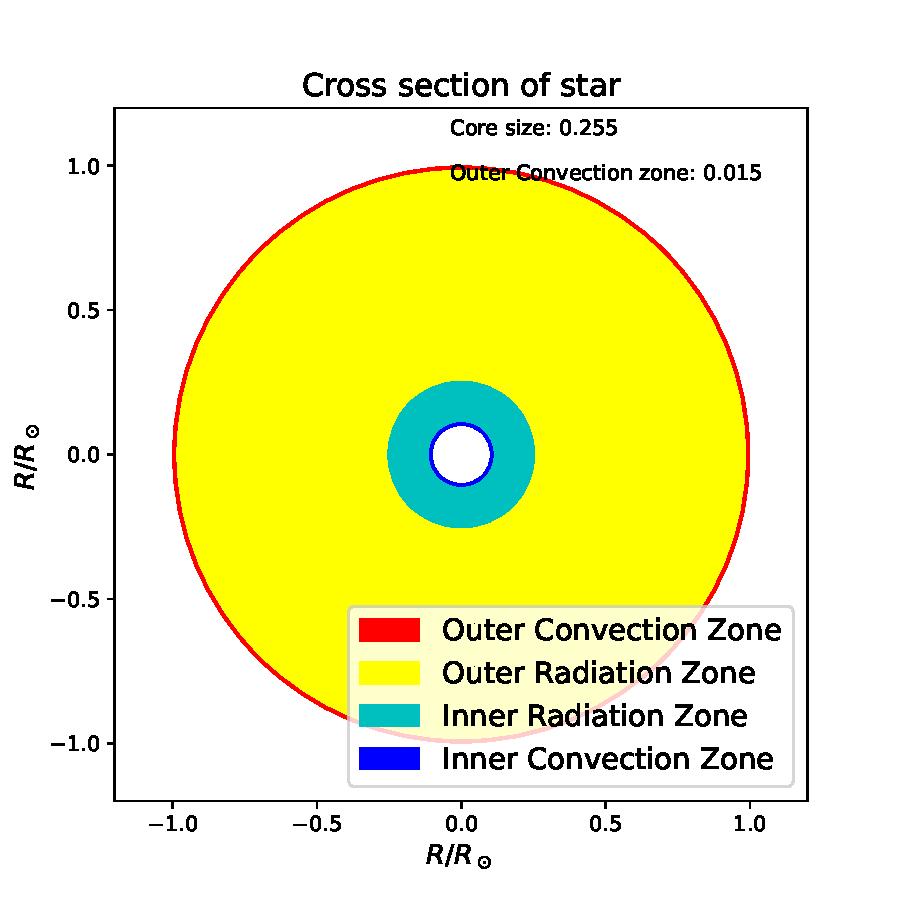
\includegraphics[width = 0.5\textwidth]{Figures/final_cross_sanity_check.pdf} 
    \label{fig_:sanity_cross}
\end{figure}

\begin{figure}[H]
    \caption{Behaviour of temperature gradients $\nabla_{stable}$, $\nabla_{ad}$ and $\nabla^*$ as function of distance to centre, with a logarithmic y-scale. Simulation ran with p=0.1}
    \centering
    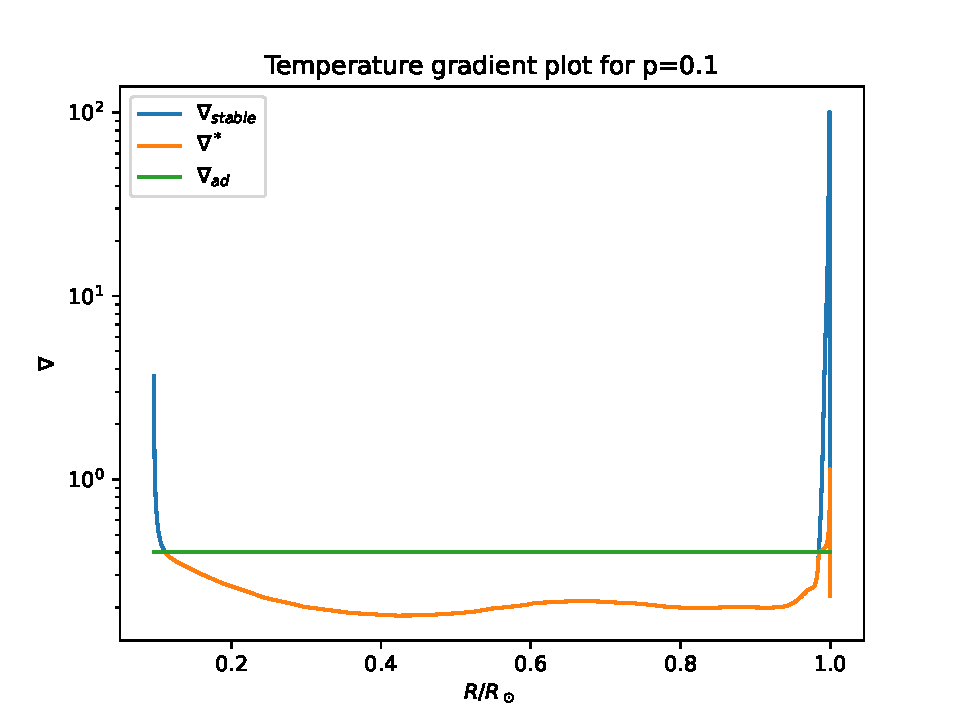
\includegraphics[width = 0.5\textwidth]{Figures/TemperatureGradients_sanity_check.pdf} 
    \label{fig_:sanity_grad}
\end{figure} 



\newpage
\subsection{Data Analysis}
\begin{figure}[H]
    \caption{Visualization of the energy transportation zones for varying values of constants. Top plots show the zones for a decrease and increase in surface density $\rho$, top center plots show decrease and increase in surface temperature T, bottom centre plots pictures the implication of decreasing the surface luminosity, and the bottom set of plots show an increase in radius affects the structure. Each plots show the core and outer convection zone sizes as fractions of the radius. Simulations ran for p=0.1}
    \centering
    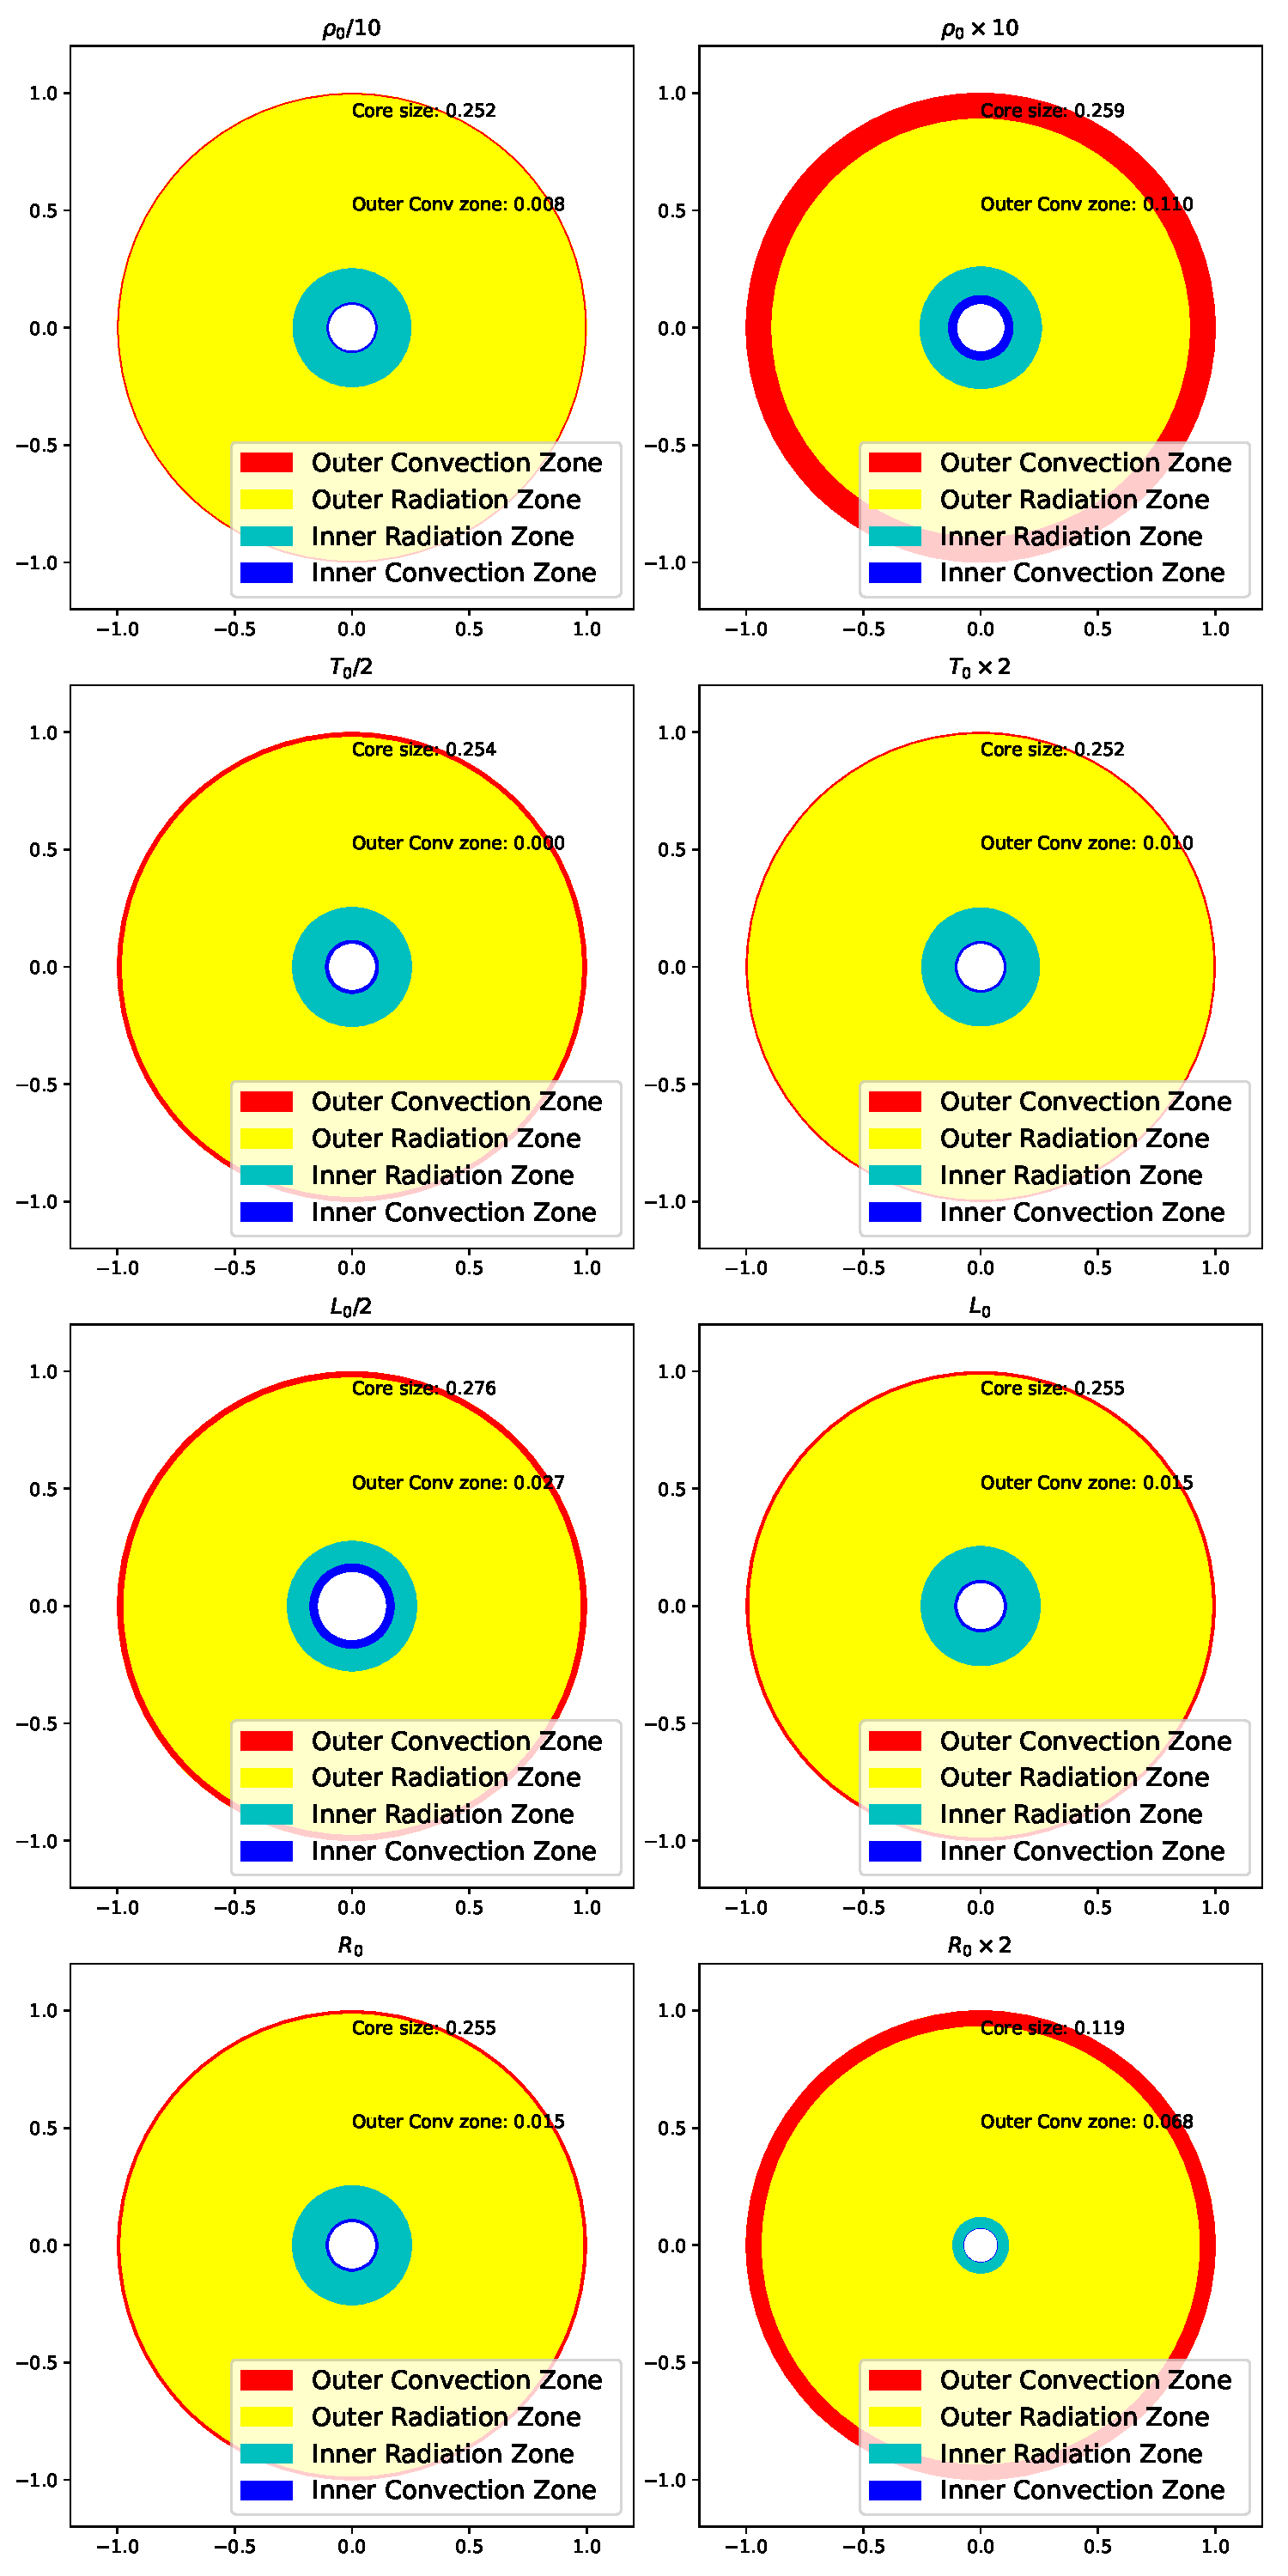
\includegraphics[width = 0.5\textwidth]{Figures/simulation_part1.pdf} 
    \label{fig:test_1}
\end{figure} 
\newpage
We use the model to investigate the implications of changing the variables defining the surface of the sun, by changing them and visualizing the structural impact of these changes in the Figure \ref{fig:test_1} and Figure \ref{fig:test_2}

\begin{figure}[H]
    \caption{Visualization of the energy transportation zones for a decrease and increase in surface pressure. Core and outer convection zone sizes shown as fractions of the radius. Simulations ran for p=0.1}
    \centering
    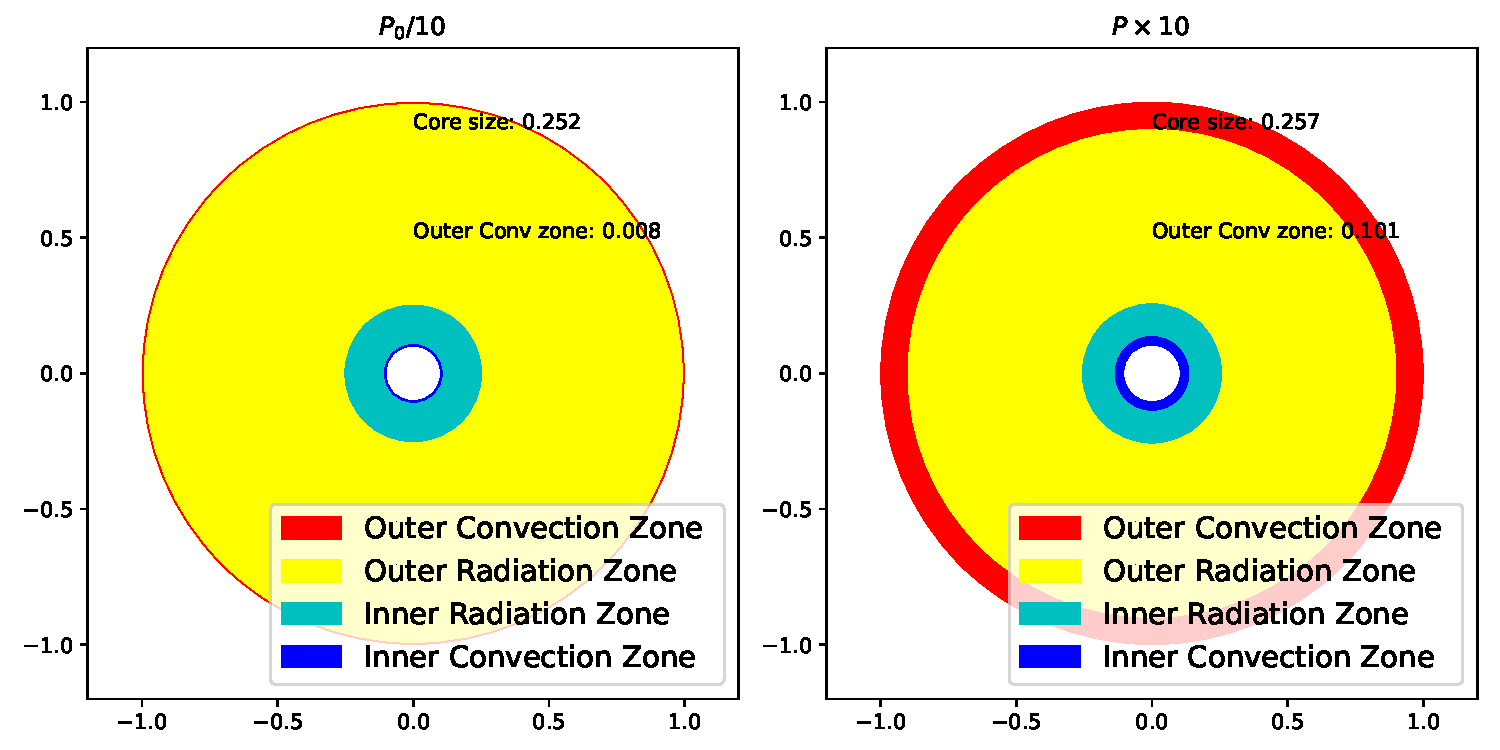
\includegraphics[width = 0.5\textwidth]{Figures/simulation_part2.pdf} 
    \label{fig:test_2}
\end{figure} 

A closer look at how the structure of the different energy-transport zones vary with varying constants is provided in the Figure \ref{fig:test_construction}. 

\begin{figure}[H]
    \caption{Construction of energy-transport zones; x-axis is the scaled radius and the y-axis visualize the zones. The zone where the outer convection is active is marked by 3 on the y-scale, outer radiation zone is marked by 2, inner radiation by 1 and the inner convection zone by 0. The scaled radius $(r=1/10)$ in which we wish the core to reach, as well as the surface $(r=1)$ is also marked to enhance the interpretability.}
    \centering
    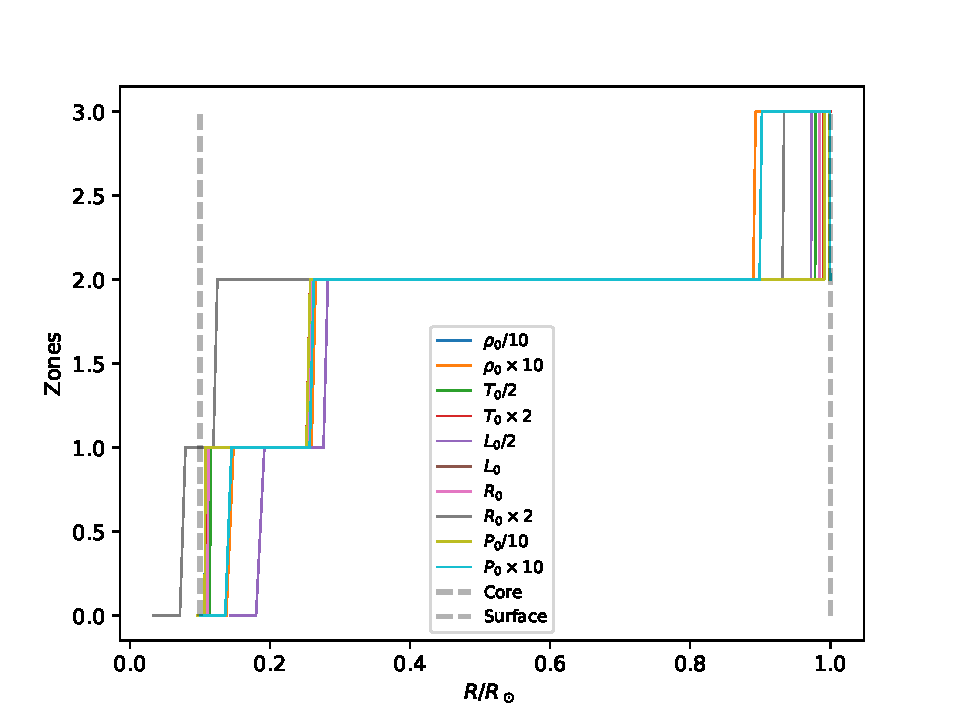
\includegraphics[width = 0.5\textwidth]{Figures/construction.pdf} 
    \label{fig:test_construction}
\end{figure} 

The combination of variables describing the surface of the star, resulting in the construction of energy transportation zones meeting the requirements set for the desired star is extracted from the Figure \ref{fig:test_1}, Figure \ref{fig:test_2} and Figure \ref{fig:test_construction}. A subsequent data analysis is performed by running a simulation using these variables, and presenting the data in plots.

\begin{figure}[H]
    \caption{Cross section plot visualizing the construction of energy transportation zones in the star, simulated with usage of the surface-defining variables  $L_0=1.7$, $R_0=1$, $M_0=1.1$, $T_0=2\times5770$, $\rho_0=70\times1.42\times 10^{-7}$, and p=0.1.  Core and outer convection zone sizes shown as fractions of the radius.}
    \centering
    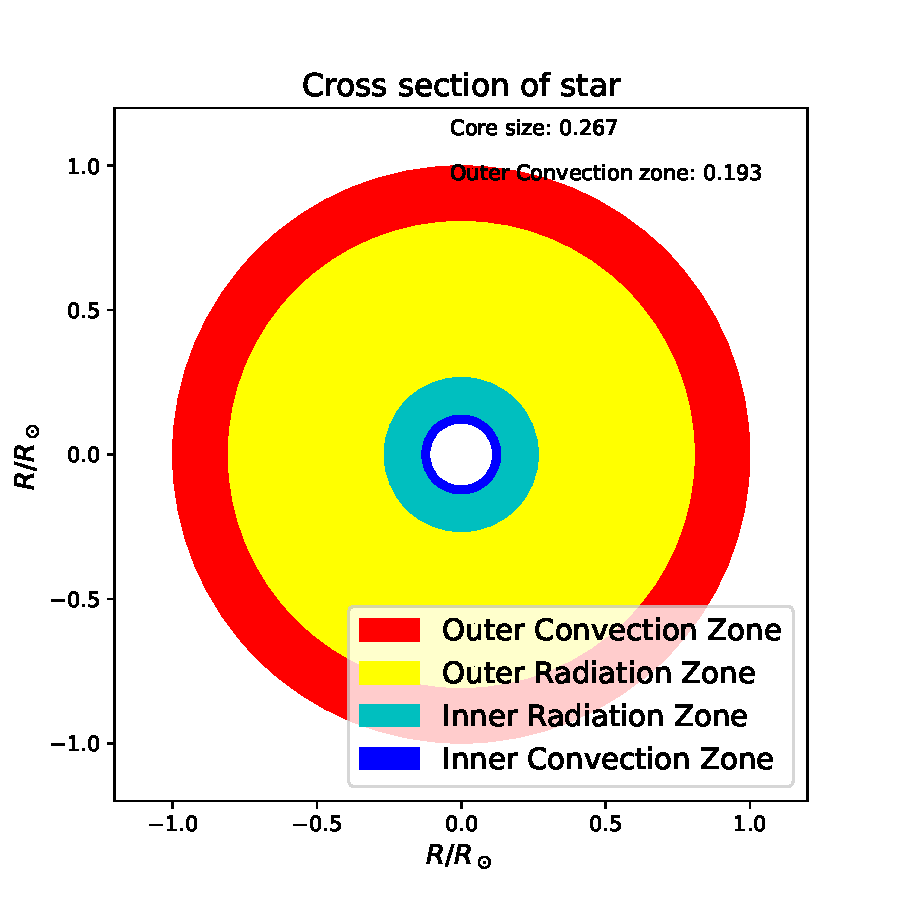
\includegraphics[width = 0.45\textwidth]{Figures/final_crossfinal.pdf} 
    \label{fig:cross}
\end{figure} 

\begin{figure}[H]
    \caption{Behaviour of temperature gradients as function of the distance from the star centre, scaled by the radius of the star. Simulation ran with usage of the surface-defining variables $L_0=1.7$, $R_0=1$, $M_0=1.1$, $T_0=2\times5770$, $\rho_0=70\times1.42\times 10^{-7}$, and p=0.1}
    \centering
    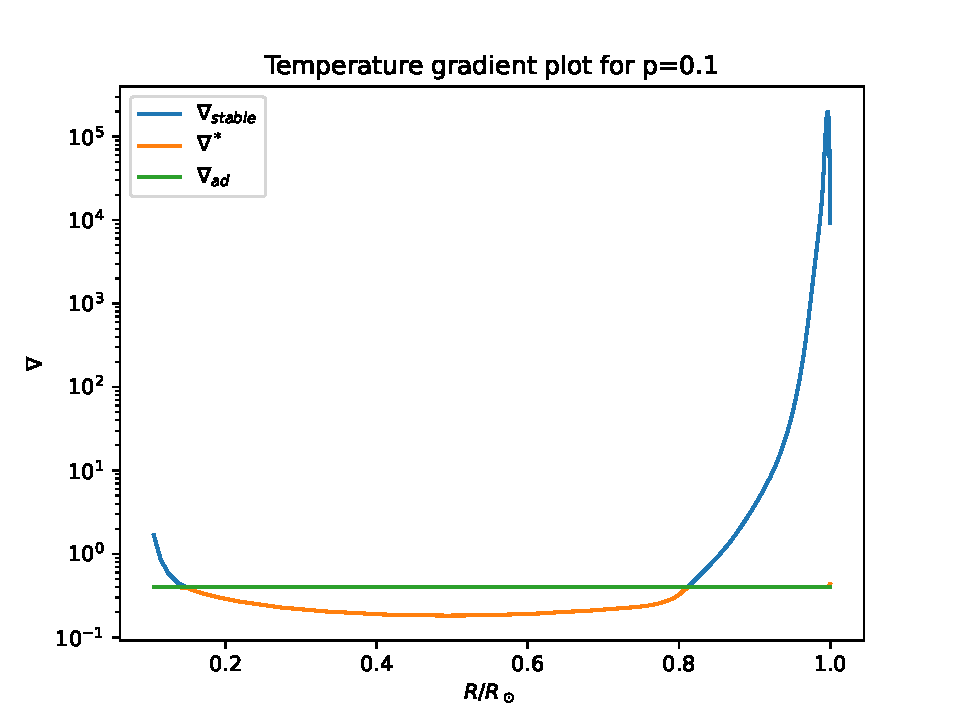
\includegraphics[width = 0.52\textwidth]{Figures/TemperatureGradientsfinal.pdf} 
    \label{fig:grad}
\end{figure} 

\newpage
\begin{figure}[H]
    \caption{The relationship between the flux of energy due to the transport of energy by radiation and the transportation by convection as a function of the distance from the star centre. Simulation ran with usage of the surface-defining variables  $L_0=1.7$, $R_0=1$, $M_0=1.1$, $T_0=2\times5770$, $\rho_0=70\times1.42\times 10^{-7}$, and p=0.1}
    \centering
    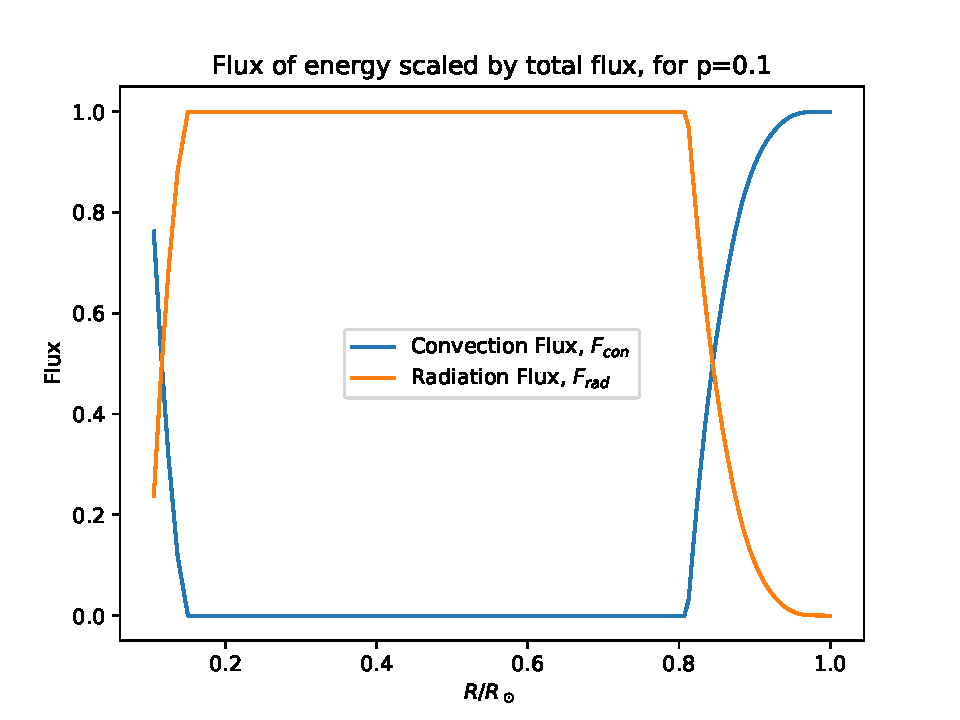
\includegraphics[width = 0.55\textwidth]{Figures/Fluxfinal.pdf} 
    \label{fig:flux}
\end{figure} 

\begin{figure}[H]
    \caption{Energy produced by the different branches of fusion PP1, PP2, PP3 and CNO, scaled by the total energy production occurring within the stellar core, as well as the total production, all as function of the distance from the centre of the star scaled by radius. Simulated with usage of the surface-defining variables $L_0=1.7$, $R_0=1$, $M_0=1.1$, $T_0=2\times5770$, $\rho_0=70\times1.42\times 10^{-7}$, and p=0.1}
    \centering
    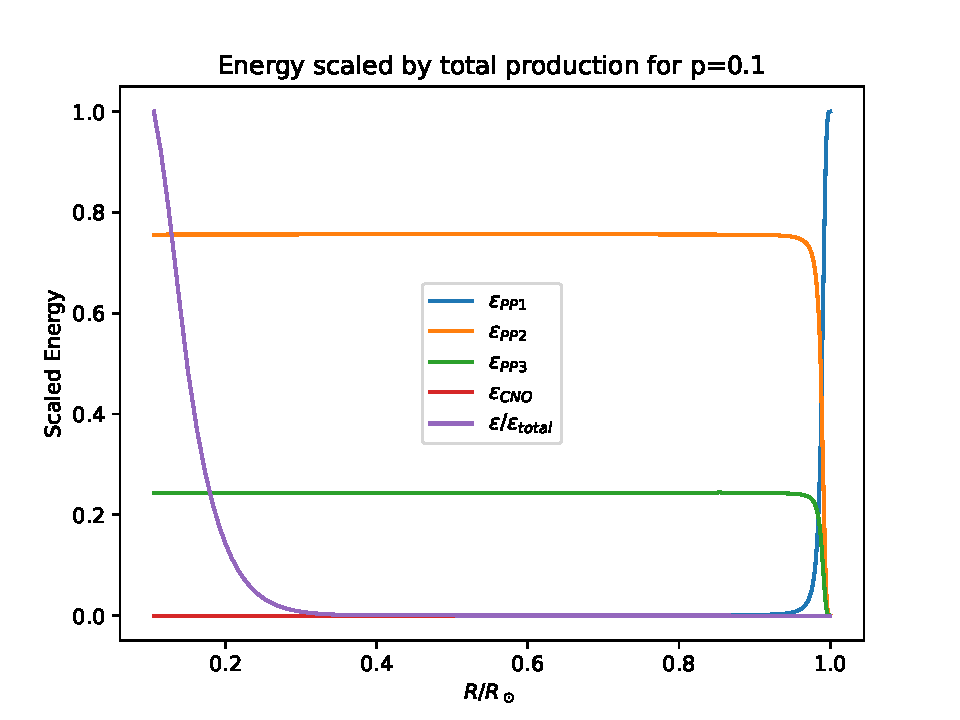
\includegraphics[width = 0.55\textwidth]{Figures/EnergyProductionfinal.pdf} 
    \label{fig:energy}
\end{figure} 

\begin{figure*}
    \caption{Evolution of the star surface-defining variables as function of the scaled distance from the centre of the star. Top left plot show the behaviour of the luminosity and mass scaled by the surface values, top right visualize the evolution of temperature, bottom left pictures the pressure with logarithmic y-scale, and bottom right shows the density also with a logarithmic scale on the y-axis - all of which are functions of the scaled distance from the star centre. Simulation ran with usage of initial variables $L_0=1.7$, $R_0=1$, $M_0=1.1$, $T_0=2\times5770$, $\rho_0=70\times1.42\times 10^{-7}$, and p=0.1}
    \centering
    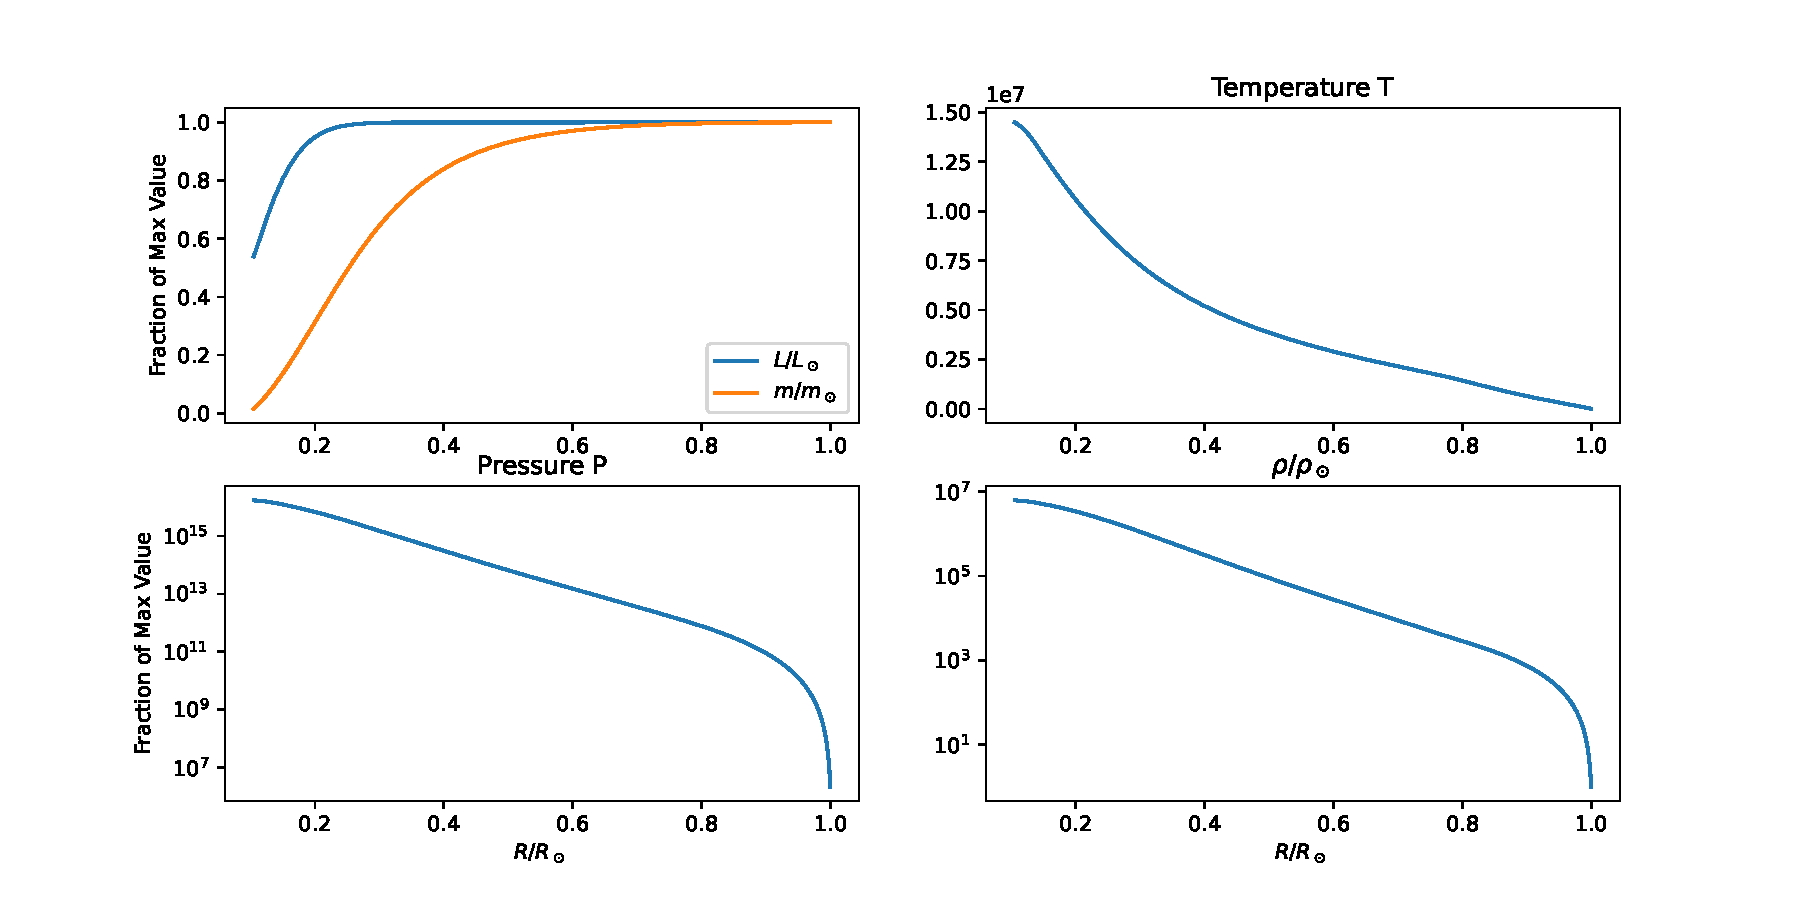
\includegraphics[width = 0.95\textwidth]{Figures/VariablesSpecialfinal.pdf} 
    \label{fig:variables}
\end{figure*} 

\newpage
The behaviour visualized in \ref{fig:cross}, Figure \ref{fig:grad} and Figure \ref{fig:flux} describe the transportation of energy and how it changes as functions of distance from centre, the Figure \ref{fig:energy} visualizes what branches of fusion are active in the different parts of the star, and the Figure \ref{fig:variables} visualizes how each of the defining variables $L, R, M, \rho, T$ and $P$ behave. 


\section{Discussion}
From the sanity checks, results extracted from Table \ref{tab:acc_kappa_sanity} one can read a very good conformity between the expected and calculated opacity by the interpolated function ; the largest relative error being $10^{-4}$. The calculated mean molecular weight is 0.618, which is a value that does not deviate far from the expected 0.6. The temperature gradients at the surface of the star shows a relationship $(\nabla_{p}= 0.2321) < (\nabla^*=0.2323) = (\nabla_{stable}=0.2323) < (\nabla_{ad} = 0.4)$. This has the physical interpretation of energy transportation due to radiation, which is not expected for a zone where energy is being transported due to convection. \\

The plotted sanity check of Figure \ref{fig_:sanity_cross} and Figure \ref{fig_:sanity_grad} agrees with the expected shapes of the temperature gradients and active zones of transportation within the sun - the cross section plot shows an empty space in the middle where r does not reach 0, small convection zones both on the inside and outside of the core, and large energy flux due to transportation by radiation for the largest part of the star. The temperature gradient confirms a relationship between the temperature gradients which varies in the same intervals of distance from the centre; first $\nabla_{ad}\leq\nabla^*<\nabla_{stable}$, indicating the convection zone. Then $\nabla^*\leq\nabla_{stable}<\nabla_{ad}$ which characterizes radiation zones. Finally, in the radius interval close to the surface, there's a peak which indicates a return to transportation by convection, before the plot finally returns a relationship indication transportation by radiation. This validates the relationship between the temperature gradients derived by the sanity check - there must be a small radiation zone at the surface of the star, which does not invalidate the accuracy of the model.  \\

%We performed a sanity check of the models calculation of a number of values within the convection zone of a star, with defining and expected values presented in Table \ref{tab:second}. The modelled values were presented in Table \ref{tab:sanity_con}, and we observe a conformity between the expected and calculated values which emphasizes the models ability to depict the energy transportation occurring in the star. Even so, there's an obvious deviation between the expected and calculated $\xi$ and $\nabla_{stable}$ which is worth commenting on, notwithstanding the ability to model the behaviour. \\
After running a simulation with defining and expected values presented in Table \ref{tab:second}, a sanity check of the models calculation of a number of values within the convection zone of a star is performed with its results presented in Table \ref{tab:sanity_con}. We observe a great conformity between the expected and calculated values which emphasizes the models ability to depict the energy transportation occurring in the star.\\




We analyse the changes in the structure of the energy transportation as a result of changes in surface defining variables, presented in the cross section plots in Figure \ref{fig:test_1} and Figure \ref{fig:test_2}; whenever we increase the surface density $\rho$, we increase the size of both convection zones, and a decrease shrinks the same zones. The change of temperature has the opposite effect; the increase leads to less transportation by convection a decrease leads to an increase. Whenever the luminosity is decreased, the empty space within the middle of the cross section plot increases, the inner convection zone decreases and the outer convection zone increases. An increase in radius reduces the empty space within the middle of the plot, decreases the size of the inner convection and radiation zones, and leads to an increase in the size of the outer convection zone. The decrease in pressure also decreases the size of both convection zones, and an increase increases the size of the convection zones. \\

These behaviours can all be explained by looking at the definitions of flux of energy due to convection Equation \eqref{eq:F_con} and radiation Equation \eqref{eq:F_rad}; whenever the surface density increases the flux of energy due to radiation decreases - explaining how the size of the associated zones also decreases. The change in pressure yields similar results due to the definition of pressure P in Equation \eqref{eq:P_sum} being defined as the sum of radial pressure and pressure from the gas itself. An increase in temperature increases the flux of energy due to radiation. We know whenever the luminosity is decreased, so does the ability for our simulation to calculate energy transportation all the way to the star centre, this due to the definition of luminosity being defined by the amount of energy radiated per second, leading to a decrease in the total flux defined by Equation \eqref{eq:flux}. A similar effect will come from changing the radius of the star; an increase in radius increases the luminosity, and leads to a subsequent ability for the surface energy to reach the centre of the star. \\

The star meeting the conditions set for the desired structure of the energy transportation zones is constructed with this information in mind, with help from the plot visualized in Figure \ref{fig:test_construction}. Increasing the density $\rho_0$ allows for the construction of a broader outer convection zone, of size 15$\%$ of the radius, and brings it to the surface of the star making it continuous. Increasing the mass has the same effects, increasing the pressure and thereby increasing the size of the convection zone. Increasing the temperature balances the huge increase of size in the convection zone as a consequence of the increase in pressure and mass, and increasing the surface luminosity allows for the temperature transportation to be modelled for a larger portion of the interval of star radius. Thereby, we choose the sets of surface-defining variables $L_0=1.7$, $R_0=1$, $M_0=1.1$, $T_0=2\times5770$, $\rho_0=70\times1.42\times 10^{-7}$.\\

%Increasing the radius allows us to both create a model where the transportation is simulated closer to the star centre, and from the Figure \ref{fig:test_construction} it is clear that this increase in radius also allows for the energy transportation within the core taking place within the interval of r where the desired core is defined. Increasing the radius, however, decreases the fraction of the total radius made up by the core, which is not ideal, and we need to balance this effect by either decreasing the luminosity, increasing the pressure or the density. 


\newpage
We run a simulation and create plots for a data analysis using  $L_0=1.7$, $R_0=1$, $M_0=1.1$, $T_0=2\times5770$, $\rho_0=70\times1.42\times 10^{-7}$. From Figure \ref{fig:cross} it is clear that this simulation returns a core of size $0.267R/R_\odot$ and a convection zone size $0.193R/R_\odot$, which meets the requirement set for the structure of energy transportation. The plots presented in Figure \ref{fig:grad} and Figure \ref{fig:flux} validates that the structure the star is as desired - the energy flux due to radiation being minimized near the surface of the star, meaning the energy transportation near the surface is due to a consecutive zone of convection. The plots of energy production presented in Figure \ref{fig:energy} show a consistent relationship between the activeness of the PP2 and PP3 branches. Closest to the surface of the star, where the temperature is the lowest, the production of the pp1 branch peaks. This is to be expected, as higher temperatures are needed for fusion of the heavier elements involved in the other branches to occur. When the scaled distance from the star centre becomes smaller than 0.2, the energy production picks up, keeping the distribution of energy production from PP2 and PP3 the same, heating up the star, but not to the point where the CNO-cycle becomes active. This does reflect the results from the data analysis performed for the energy production in the Project 1 report - the  CNO-cycle only becomes an active form of energy production when the temperature reaches $T=10^8K$, which is not the case for the modelled star. Since the temperature is very high all the way from the core of the star, and to the surface of the star the steadiness of the energy production from PP2 and PP3 branches in Figure \ref{fig:energy} are verified. \\


\newpage
The Figure \ref{fig:variables} shows how the relation between pressure and density is consistent,which would be expected by looking at Equation \eqref{eq:P_sum}, which describes the total pressure as a sum of that from the radiation and that of the gas itself - density dependent. It is also clear that the star temperature increases exponentially as the distance from the centre decreases, as expected from the interpretation of the behaviour of energy produced visualized in Figure \ref{fig:energy}. Furthermore, we manage to keep the luminosity consistent, and the mass distribution decreasing before it hits zero near the centre of the star.


\section{Conclusion}
The model meets a great level of conformity with what is expected, and returns relative errors and behaviours that is expected. The implications of changing the surface-defining variables are tested, visualized and deliberated upon, and subsequently used as grounds in defining a star meeting the requirements set for the desired structure. We perform an analysis for the behaviour of relevant variables, and see that it does model energy transportation in the way we wanted, and reflects the expected behaviours. \\


\section{Reflection}
This exercise has taught me everything I know about the transportation of energy within a star. The model I created passed my sanity checks, and was deemed accurate, which is a result I only reached after a lot of deliberating on how to structure my code, and evolve the calculations of variables from the surface and to the centre of the star. At first, it was an overwhelming amount of theory needed in order to develop the model, which at first led to some frustration. I reduced the \textit{"overwhenming-ness"} of the task by implementing each of the variables as method-functions in the class for energy production, and eventually managed to get a grip over the theory. A lot of confusion also stemmed from the lack of a total energy production calculation in my class that defined energy production by fusion in the core, which I solved by redefining a method from this class directly in the new python document.

\bibliographystyle{plain}
\bibliography{references}

\cleardoublepage
\end{document}